\documentclass[margin=0px]{article}

\usepackage{listings}
\usepackage[utf8]{inputenc}
\usepackage{graphicx}
\usepackage{float}
\usepackage[a4paper, margin=1in]{geometry}
\usepackage{amsthm}

\renewcommand{\figurename}{ábra}
\newenvironment{tetel}[1]{\paragraph{#1 \\}}{}

% A dokument itt kezdődik

\title{Záróvizsga tételsor \\ \large 8. Programfejlesztési modellek}
\date{}
\author{Dobreff András}

\begin{document}
	\maketitle
	
	\begin{tetel}{Programfejlesztési modellek}
			Nagy rendszerek fejlesztési fázisai, kapcsolataik. Az objektumelvű modellezés nézetrendszerei. Statikus modell (osztálydiagram, objektumdiagram). Dinamikus modell (állapotdiagram, szekvenciadiagram, együttműködési diagram, tevékenységdiagram). Használati esetek diagramja.
	\end{tetel}
	
	\section{Nagy rendszerek fejlesztési fázisai, kapcsolataik}
	
	\subsection{Fejlesztési fázisok}
		\begin{enumerate}
			\item A probléma megoldásának előzménye
			
				Egy probléma megoldása előtt meg kell vizsgálni a megvalósíthatóságát, és annak mikéntjét. Eredmény: \textit{Megvalósíthatósági tanulmány}, mely a következőkre válaszol:
				\begin{itemize}
					\item Erőforrások (hardver, szoftver, szakember)
					\item Költségek
					\item Határidő
					\item Üzemeltetés
				\end{itemize}
			\item Követelmények leírása
			
				Rendszerint iteratív módon állítjuk elő, és a prototípust használjuk a finomításra (ábra \ref{fig:kovetelmenyleiras}).
				
				\begin{figure}[H]
						\centering
						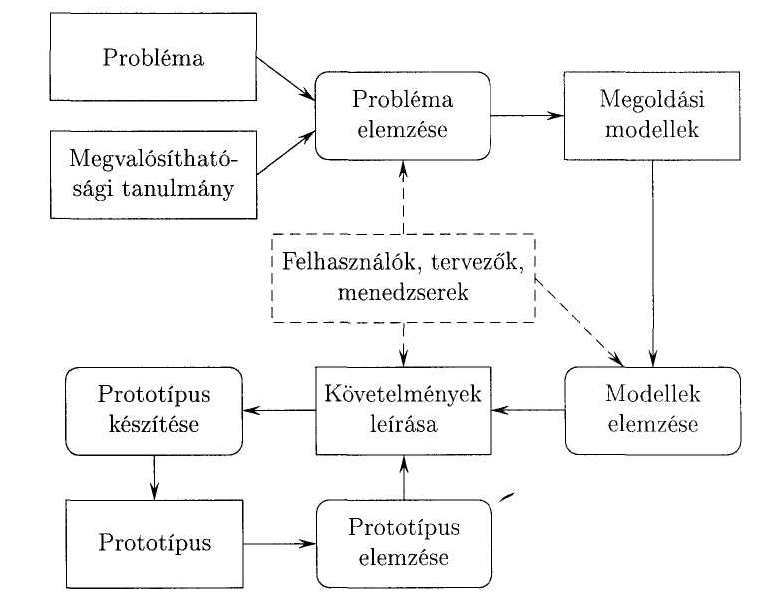
\includegraphics[width=0.5\textwidth]{img/kovetelmenyleiras.png}
						\caption{Követelményleírás elkészítésének folyamata}
						\label{fig:kovetelmenyleiras}
				\end{figure}
				
				Követelmények leírásának tartalma:
				
				\begin{itemize}
					\item Probléma
					\item Korlátozó tényezők (hardver, szoftver, stb.)	
					\item Elfogadható megoldás
				\end{itemize}
				
				Követelmények leírásának fajtái:
				
				\begin{itemize}
					\item Funkcionális követelmények
					
					A rendszer szolgáltatásainak, leképzéseinek leírása:
						\begin{itemize}
							\item Elindítás formája
							\item Bemenő adatok (és azok megadásának formája)
							\item Igénybevétel előfeltétele, korlátozások
							\item Szolgáltatás kezdeményezésére a válasz, eredmények
							\item Válasz megjelenési formája
							\item Bemenő adatok és válasz közti reláció
						\end{itemize}
					\item Nem funkcionális követelmények
					
					A nem funkcionális követelményeket rendszerint három osztályba soroljuk: a termék követelményei, menedzselési követelmények, külső követelmények. Az osztályokat tovább lehet bontani (ábra \ref{fig:nemfunkckov}).
						\begin{figure}[H]
							\centering
							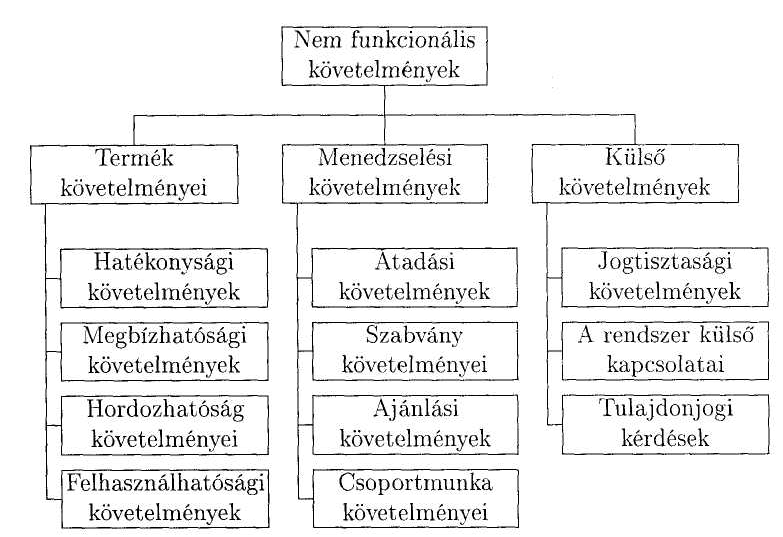
\includegraphics[width=0.5\textwidth]{img/nemfunkckov.png}
							\caption{Nem funkcionális követelmények osztályozása}
							\label{fig:nemfunkckov}
						\end{figure}
				\end{itemize}
				
			\item Követelmények elemzése és prototípus

				A következőket kell megvizsgálni:
				\begin{itemize}
					\item Önmagában jó-e a követelmények leírása?
						\begin{itemize}
							\item Konzisztens (nincs ellentmondás)
							\item Komplett (teljes)
						\end{itemize}
						\item Validáció vizsgálat
						
						(Megfelel-e a felhasználó által elképzelt problémának?)
						
						\item Megvalósíthatósági vizsgálat
						
						(A követelményeknek megfelelő megoldás megvalósítható-e?)
						
						\item Tesztelhetőségi vizsgálat
						
						(A követelmények úgy vannak-e megfogalmazva, hogy azok tesztelhetők?)
						
						\item Nyíltság kritériumainak vizsgálata.
						
						(A követelmények nem mondanak-e ellent a módosíthatóság, a továbbfejleszthetőség
						követelményének?)
				\end{itemize}
				
				A követelmények elemzésének egyik eszköze a prototípus-készítés.
				A prototípus magas szintű programozási környezetben létrehozott, a
				külső viselkedés szempontjából helyes megoldása a problémának.
			\item Programspecifikáció
			
				A programspecifikáció a következő kérdésekre kell, hogy válaszoljon a
				követelmények leírása alapján:
				
				\begin{itemize}
					\item Mik a bemenő adatok? (Forma, jelentés, megjelenés.)
					\item Mik az eredmények? (Forma, jelentés, megjelenés.)
					\item Mi a reláció a bemenő adatok és az eredmény adatok között?
				\end{itemize}
			\item Tervezés
			
				A tervezés során a következő kérdésekre adjuk
				meg a választ:
				\begin{enumerate}
					\item Statikus modell
						\begin{itemize}
							\item Rendszer szerkezete
							\item Programegységek, azok feladata és kapcsolata
						\end{itemize}
					\item Dinamikus modell
					\begin{itemize}
						\item Hogyan oldja meg a rendszer a problémát?
						\item Milyen egységek működnek együtt?
						\item Milyen üzenetek játszódnak le?
						\item Rendszer és egységek állapotai
						\item Események (melyek hatására állapotváltás történik)
					\end{itemize}
					
					\item Funkcionális modell
					\begin{itemize}
						\item Milyen adatáramlások révén valósulnak meg a szolgáltatások?
						\item Milyen leképezések játszanak szerepet az adatáramlásokban?
						\item Mik az ajánlások az implementáció számára?
						\begin{itemize}
							\item Implementációs stratégiára vonatkozó ajánlás.
							\item Programozási nyelvre vonatkozó előírás, ajánlás.
							\item Tesztelési stratégiára vonatkozó ajánlás.
						\end{itemize}
					\end{itemize}
				\end{enumerate}
				
				A gyakorlatban két tervezési módszer terjedt el:
				\textit{procedurális} és a \textit{objektumelvű}
				
				(\textit{procedurális}: megvalósítandó funkciókból, műveletekből indulunk ki, és ezek alapján bontjuk fel a rendszert kisebb összetevőkre, modulokra\\
				\textit{objektumelvű}: a rendszer funkciói helyett az
				adatokat állítjuk a tervezés középpontjába. A rendszer által használt
				adatok felelnek meg majd bizonyos értelemben az objektumoknak.)
			
			\item Implementáció
			
				Fontos szempontok:
				\begin{itemize}
					\item Reprezentáció (Adatok ábrázolása)
					\item Események leképezések megvalósítása
	
						Algoritmusok és optimalizálások
				\end{itemize}
				
				Az implementáció egyik alapvető kérdése az implementációs stílus.
				A jó programozási stílus néhány fontos eleme:
				\begin{itemize}
					\item absztrakció különböző szintjeinek alkalmazása
					\item öröklődési technika használata, absztrakciós szintek hierarchikus
					rendszere
					\item absztrakciós szintekre bontás osztályon belül (deklaráció + megvalósítás)
					\item korlátolt láthatóság;
					\item információ elrejtés (information hiding);
					\item információ beburkolás (encapsulation).
				\end{itemize}
				
			\item Verifikáció, validáció
			
			A rendszer eleget tesz-e a vele szemben támasztott elvárásoknak?
			
			Verifikáció: a specifikációszerinti helyesség igazolása
			
			Validáció: Minőségi előírások teljesítése (robosztusság hatékonyság, erőforrásigény)
			
			Ennek folyamata: tesztelés, melynek szakaszai:
			\begin{itemize}
				\item Egységteszt
				\item Rendszerteszt 
			\end{itemize}
			A tesztelésnek két módja lehet:
			\begin{itemize}
				\item fekete doboz - Csak a maguknak a hibáknak a felderítése
				\item fehér doboz - Hibák helyének felderítése 
			\end{itemize}
			
			\item Rendszerkövetés és karbantartás (maintenance)
			
			Karbantartás: Üzemebe helyezés után szükségessé váló szoftver jellegű munkák [pl.: rejtett hibák kijavítása, adaptációs munkák (új harver-, szoftverkörnyezet), továbbfejlesztési munkák]
			
			Rendszerkövetés: a felhasználókkal való kapcsolattartás menedzsment jellegű, dokumentációs feladatai [pl.: konfigurációk nyilvántartása, verziók menedzselése, dokumentáció menedzselése]
			
			\item Dokumentáció
			
			Egy nagy méretű program önmagában nem tekinthető szoftverterméknek
			dokumentáció nélkül. Egy jó dokumentáció a következőképp épül fel.
			\begin{itemize}
				\item Felhasználói leírás
					\begin{itemize}
						\item Feladatleírás
						\item Futtató környezet
						\item Fejlesztések, verziók
						\item Installálás
						\item Használat
						\item Készítők
					\end{itemize}
				\item Fejlesztői leírás
					\begin{itemize}
						\item Modulok (és azok szerkezete)
						\item Osztályok (és azok kapcsolata)
						\item Rendszer dinamikus viselkedése
						\item Osztályok implementálása (adatszerkezetek, sablon osztályok)
						\item Tesztelés
					\end{itemize}
			\end{itemize}	
		\end{enumerate}
		
		\subsection{Fejlesztési fázisok kapcsolatai}
		
		A fejlesztési fázisok leírására többféle modellt használhatunk
		\begin{enumerate}
			\item Vízesés modell
			
				Az egyes fázisok egymást követik, a
				módosítások a futtatási eredmények ismeretében történnek. Egy bizonyos
				fázisban elvégzett módosítás az összes rákövetkező fázist is érinti.
				
				\begin{figure}[H]
					\centering
					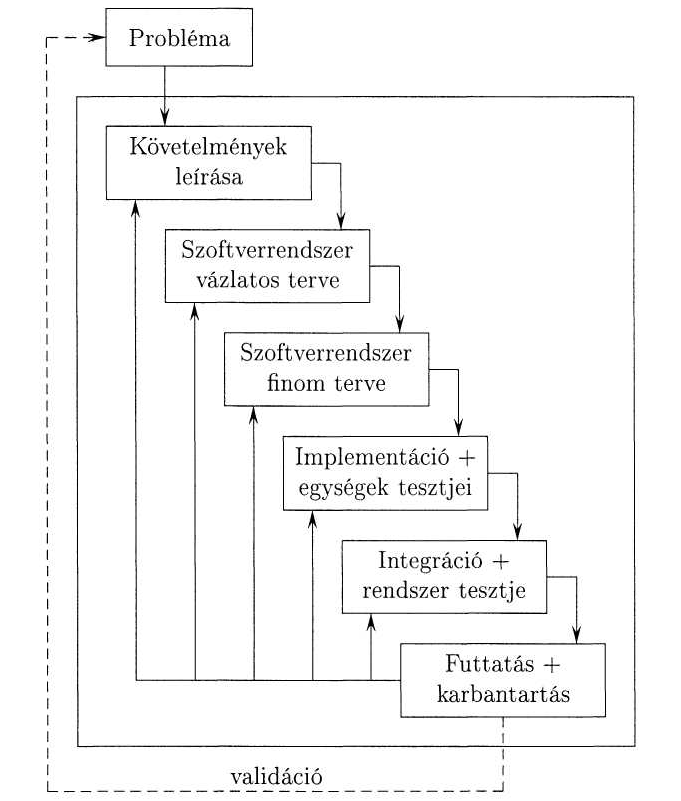
\includegraphics[width=0.5\textwidth]{img/vizeses.png}
					\caption{Vízesés modell}
					\label{fig:vizeses}
				\end{figure}
				
				Hárányai: 
					\begin{itemize}
						\item Új szolgáltatás minden fázison módosítást igényel
						\item Validáció az egész életciklus megismétlését követelheti meg
					\end{itemize}
			\item Evolúciós modell
			
				A megoldást közelítő verzióinak, prototípusainak sorozatát
				állítjuk egymás után elő, és így haladunk lépésenként egészen a végleges
				megoldásig. Ennek során egy verzió elkészítésekor a specifikáció, a fejlesztés és a validáció párhuzamosan történik.
				
				\begin{figure}[H]
					\centering
					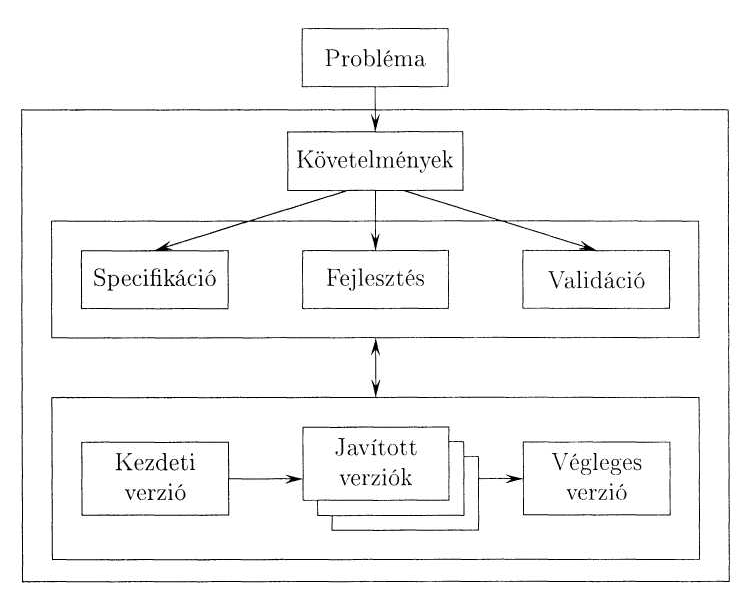
\includegraphics[width=0.5\textwidth]{img/evolucios.png}
					\caption{Evolúciós modell}
					\label{fig:evolucios}
				\end{figure}
				
				Hárányai: 
				\begin{itemize}
					\item Nehéz a projekt áttekintése
					\item A gyors fejlesztés rendszerint a dokumentáltság rovására megy.
				\end{itemize}
			\item Boehm-féle spirális modell
			
				Ez a modell egy iterációs modell. Az iteráció a spirális egy
				fázisával modellezhető, amely négy szakaszra bontható:
				\begin{enumerate}
					\item Célok, utak, alternatívák, korlátozások definiálása
					\item Kockázatelemzés, stratégia kidolgozás
					\item Feladat megoldása, validáció
					\item Következő iteráció megtervezése
				\end{enumerate}
				
				\begin{figure}[H]
					\centering
					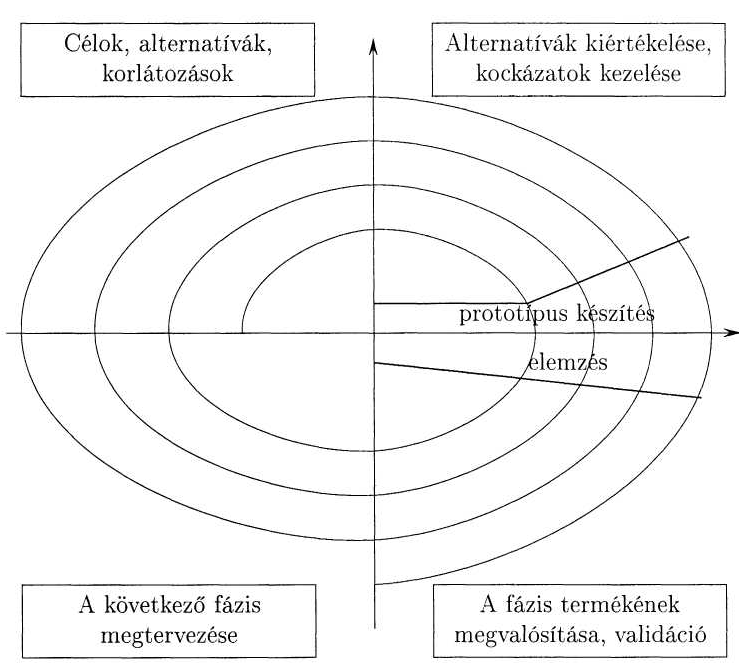
\includegraphics[width=0.5\textwidth]{img/spiral.png}
					\caption{Evolúciós modell}
					\label{fig:spiral}
				\end{figure}
				
				Hárányai: 
				\begin{itemize}
					\item A modell alkalmazása általában munkaigényes, bonyolult feladat.
					\item A projekt kidolgozásához szükséges szakembereket nem könnyű
					gazdaságosan foglalkoztatni.
				\end{itemize}
		\end{enumerate}
		
	\section{Az objektumelvű modellezés nézetrendszerei}
	
		\textbf{Objektumelvű programozás} = adatabsztrakció + absztrakt adattípus + típusöröklődés
		\begin{itemize}
			\item Absztrakció
			
				Programozás adott szintjén a megoldás szempontjából
				lényegtelen részletek elhanyagolása.
				
			\item Adattípus
				
				Az adattípus egy $ (A,F) $ rendezett pár, ahol $ A $ az adatok halmaza $ F $ pedig a műveletek véges halmaza. ($ \forall f \in F : f:A^n \rightarrow A $) Létezik egyszerű és összetett adattípus.\\
				\textbf{Típusosztály:} A típus komplex leírása, mely az adott adattípus \underline{absztrakt} (PAR + EXP) és \underline{konkrét} (IMP + BODY) leírását szolgálja. Tehát:\\\\
				Típusosztály = (PAR, EXP, IMP, BODY), ahol:\\
				PAR = \textless paraméterek tulajdonságai \textgreater\\
				EXP = \textless típusobjektumok halmaza és műveltei neve, szintaktikája, szemantikája \textgreater\\
				IMP = \textless más osztályból átvett szolgáltatások \textgreater\\
				BODY = \textless típusosztály ábrázolása, megvalósítása \textgreater\\
				
			\item Típusöröklődés
				
				A típusöröklődés két fő formája: \textit{specializáció} és  \textit{újrafelhasználás}
				\begin{enumerate}
					\item A subclass átveszi az absztakt tulajdonságokat és azt az export részben használja fel
					\item Típushalmaz, paraméterhalmazok, műveletek nevei átdefiniálódhatnak.
					\item subclass típushalmaza = superclass típushalmaza
				\end{enumerate}
				 
				 A specializáció következményei:
				 \begin{itemize}
				 	\item polimorfizmus
				 	
					 	Minden változónak két típusa van: \textit{statikus} (deklaráció során kapott) és \textit{dinamikus} (deklaráció pillanatában megegyezik a statikussal, de később megváltozhat, ha egy superclass példánynak adunk értékül egy subclass példányt)
				 	\item dinamikus kötés
				 	
					 	A dinamikus típusnak megfelelő kiszámítási szabály hozzárendelése a függvényhez attribútumhoz, a végrehajtás pillanatában
				 \end{itemize}
				\paragraph{Nézetrendszerek}
				\begin{itemize}
					\item használati szempont
					
						Kinek nyújt a rendszer szolgáltatást? (Személyek vagy más rendszerek, programok)
						
					\item Szerkezetei strukturális, statikus szempont
					
						Milyen egységek vannak, ezeknek mi a feladata, és hogyan kapcsolódnak egymáshoz?
						
					\item Dinamikus szempont
					
						Az egyes részegységek hogyan viselkednek, milyen állapotokat vesznek fel, azokat milyen események hatására váltják? Milyen az egységek között együttműködés mechanizmusa? Időben hogyan játszódnak le közöttük az üzentek?
						
					\item Implementációs szempont
					
						Milyen szoftverkomponensek, és azok között milyen kapcsolatok vannak?
						
					\item Környezeti szempont
					
						A rendszer milyen hardver és szoftver erőforrást igényel a megoldás során?
				\end{itemize}
		\end{itemize}
	\section{Statikus modell (osztálydiagram, objektumdiagram)}
		\subsection{Osztáldiagram}
			A megoldás szerkezetét leíró összefüggő gráf, melynek csomópontjaihoz az osztályokat, éleihez pedig az osztályok közötti relációkat (öröklődés, asszociáció, aggregáció, kompozíció) rendeljük.
			
			\noindent
			A rendszerhez csak egy osztálydiagram tartozik.
			
			\begin{description}
				\item[Osztályok] \hfill \\
				
				Egy osztály a következőképp néz ki:
				\begin{figure}[H]
					\centering
					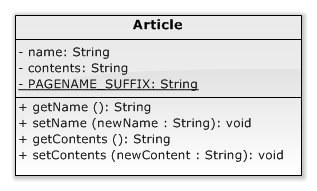
\includegraphics[width=0.4\textwidth]{img/osztaly.png}
					\caption{Osztály}
				\end{figure}
				
				Az osztályt leíró téglalap 3 részre van osztva.
					\begin{itemize}
						\item Az első részbe az osztály neve kerül.
						
						Ha az osztály absztrakt, a nevét dőlt betűvel írjuk.
						
						\item A második részbe az osztály attribútumai kerülnek.
						
						Az attribútum formátuma: \textit{Attribútumnév : Típus}
						A statikusságot aláhúzással jelöljük.
						Az attribútumok láthatóságát is fel lehet tüntetni: \textit{ publikus (+), privát (-), védett (\#)}
						
						\item A harmadik részbe az osztály metódusai kerülnek.
						
						A metódusok formátuma: \textit{Metódusnév(Paraméterlista):Visszatérési érték}, ahol a paraméterlista \textit{Paraméternév:Típus} fomrátumú paraméterekből áll.
						Absztraktságot, statikusságot, és láthatóságot az előzőekben leírtakkal azonosan jelöljük.
 					\end{itemize}
 				\item[Osztályok közötti kapcsolatok:] \hfill \\
 					
 					\begin{itemize}
 						\item öröklődés
	 						
	 						Két osztály közötti absztrakciós kapcsolatot jelöl
	 						\begin{figure}[H]
	 							\centering
	 							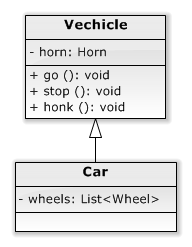
\includegraphics[width=0.2\textwidth]{img/oroklodes.png}
	 							\caption{Öröklődés}
	 						\end{figure}
	 						
 						\item asszociáció
	 						
	 						Ez a legáltalánosabb reláció két osztály között. Az asszociáció két osztály
	 						közötti absztrakt reláció, amely kétirányú társítást fejez ki. A
	 						reláció absztrakt volta azt jelenti, hogy a reláció konkretizálása osztályok
	 						objektumainak összekapcsolásában valósul meg.
	 						
	 						Az asszociációnak lehet:
	 						\begin{itemize}
	 							\item Neve, azonosítója
	 							\item Iránya
	 							\item Multiplicitása 
	 							
	 							Akár egy érték, akár intervallum. A * szimbólum kitüntett szerepet kap, jelentése: bármennyi, akár nulla is. (Pl: 3, 1..4, 5..*, *)
	 							\item Szerepe
	 							\item Navigálhatósága 
	 							
	 							A társított osztályok közül csak az egyik ismeri a másikat. (Ha nem tüntetjük fel, kölcsönös elérhetőséget feltételezünk) 
	 							
		 						\begin{figure}[H]
		 							\centering
		 							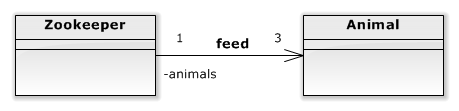
\includegraphics[width=0.5\textwidth]{img/asszociacio.png}
		 							\caption{Asszociáció}
		 						\end{figure}	
	 						\end{itemize}
	 					\item aggregáció
		 					
		 					Az aggregáció egy speciális asszociáció, mely egész-rész kapcsolatot fejez ki. Azonban ha két osztály között aggregációs reláció áll fenn, a két osztály objektumai egymástól függetlenül is létezhetnek (Ezt un. laza tartalmazási relációnak nevezik) A relációt jellemzi ezen kívül a tranzitivitás, és a közös attribútumok illetve szolgáltatások. Különböző aggregátumoknak lehetnek közös komponenseik.
		 						\begin{figure}[H]
		 							\centering
		 							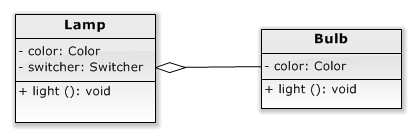
\includegraphics[width=0.5\textwidth]{img/aggregacio.png}
		 							\caption{Aggregáció}
		 						\end{figure}
 						\item kompozíció
 						
		 					A kompozíció egy speciális aggregáció, mely \textit{fizikai} tartalmazást jelöl. Nem jellemzi többé az objektumok független létezése, a két objektum egyszerre jön létre és szűnik meg. Tehát a tartalmazó objektumnak gondoskodnia kell a tartalmazott létrehozásáról és megszüntetéséről. Egy komponens legfeljebb egy tartalmazó \underline{objektumhoz} tartozhat. A kompozíciós kapcsolat és az attribútum jellegű kapcsolat két objektum között szemantikailag azonos.
			 					\begin{figure}[H]
			 						\centering
			 						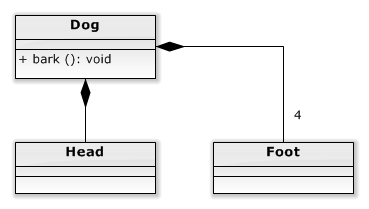
\includegraphics[width=0.4\textwidth]{img/kompozicio.png}
			 						\caption{Kompozíció}
			 					\end{figure}
 					\end{itemize}
			\end{description}
			
		\subsection{Objektumdiagram}
			Az objektumdiagram egyszeresen összefüggő gráf, amelynek csomópontjaihoz az objektumokat, éleihez pedig az objektumok közötti összekapcsolásokat rendeljük.
			
			A rendszerhez különböző időpillanatokban más-más objektumdiagram tartozhat. (Viszont mindegyiknek meg kell felelnie az osztálydiagramnak)
			
			\begin{description}
				\item[Objektumok] \hfill \\
					Az objektumokat az osztályokhoz hasonlóan egy téglalap írja le. Egy ilyen téglalapnak két része van. Az első részben az objektum neve (opcionális) és típusa található a következő formátumban: \textit{Objektumnév : Típus}, melyet aláhúzással tarkítunk. A második részbe az objektum attribútumai és azok értékei kerülhetnek, a következő formátumban: \textit{Attribútumnév=érték}.
						\begin{figure}[H]
							\centering
							\includegraphics[width=0.2\textwidth]{img/objektum.png}
							\caption{Objektum}
						\end{figure}
				\item[Objektumok közötti kapcsolatok] \hfill \\
					Az objektumokat összekötő relációk az osztálydiagramon lévőkkel megegyezőek (Öröklődésnek ezen a szinten nincs értelme):
						\begin{itemize}
							\item asszociáció
								\begin{figure}[H]
									\centering
									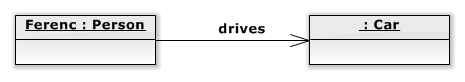
\includegraphics[width=0.5\textwidth]{img/asszociacio2.png}
									\caption{Asszociáció}
								\end{figure}
							\item aggregáció
								\begin{figure}[H]
									\centering
									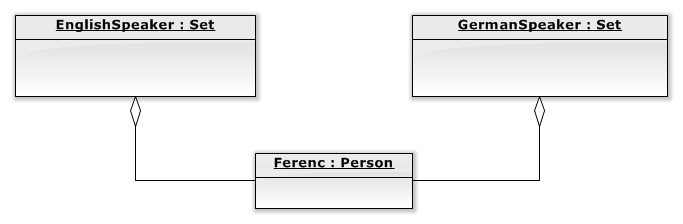
\includegraphics[width=0.7\textwidth]{img/aggregacio2.png}
									\caption{Aggregáció}
								\end{figure}
							\item kompozíció
								\begin{figure}[H]
									\centering
									\includegraphics[width=0.5\textwidth]{img/kompozicio2.png}
									\caption{Aggregáció}
								\end{figure}
						\end{itemize}
			\end{description}
	\section{Dinamikus modell (állapotdiagram, szekvenciadiagram,\\ együttműködési diagram, tevékenységdiagram)}
		
		\subsection{Állapotdiagram}
			Az állapotdiagram egy összefüggő irányított gráf, amelynek csomópontjaihoz az állapotokat rendeljük, éleihez pedig az eseményeket. (Két csúcs között több állapotátmenetet is jelölhetünk, hiszen több esemény hatására is létrejöhet)
			\begin{description}
				\item[Állapot] \hfill \\
					Az objektum állapotát az attribútumok konkrét értékeinek n-esével jellemezzük.
					
					Az állapotnak van azonosítója, mely legtöbbször az állapot neve (de lehet maga az invariáns, vagy az attribútumok konkrét értéke). Az állapotot esemény hozza létre és szünteti meg. Az állapot mindaddig fennmarad, míg az attribútumok kielégítik az állapotot leíró invariánst. Az állapotot egy lekerekített téglalappal jelöljük, melyben az azonosítót tüntetjük fel.
					
					Speciális (rendszeren kívüli) állapotok: Kezdőállapot, Végállapot
				\item[Esemény] \hfill \\
					Eseménynek nevezzük azt a tevékenységet, történést, amely valamely objektum állapotát megváltoztatja.
					
					Az esemény lehet paraméteres vagy paraméter nélküli, és lehet előfeltétele. Az események között sorrendiség áll fent, így egy esemény lehet megelőző eseménye. Egy eseményt a következőképp írhatunk le:\\
					\textless esemény \textgreater (\textless paraméterek\textgreater)[\textless feltétel\textgreater]/\textless megelőző esemény\textgreater
					
					Az eseményeket az állapotok közötti állapotátmenetekre írjuk.
					\begin{figure}[H]
						\centering
						\includegraphics[width=0.5\textwidth]{img/plane.png}
						\caption{Repülőgép állapotgépe}
					\end{figure}
			\end{description}
		\subsection{Szekvenciadiagram}
			A szekvencia diagram az objektumok közötti üzenetváltások időbeli menetét
			szemlélteti.
			\begin{description}
				\item[Osztályszerep] \hfill \\
					Az osztály szerepét olyan egy vagy több objektum testesíti meg, melyek az üzenetküldés szempontjából konform módon viselkednek.
				\item[Osztályszerep életvonal] \hfill \\
					Az életvonal az osztályszerep időben való létezését jelenti.
					\begin{figure}[H]
						\centering
						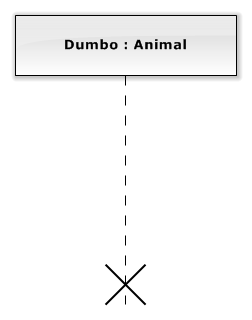
\includegraphics[width=0.3\textwidth]{img/eletvonal.png}
						\caption{Életvonal}
					\end{figure}
				\item[Aktivációs életvonal] \hfill \\
					Az aktivációs életvonal azt az állapotot jelenti, amikor az osztályszerep megtestesítői műveleteket hajtanak végre, vagy más objektumok vezérlése alatt állnak.
					\begin{figure}[H]
						\centering
						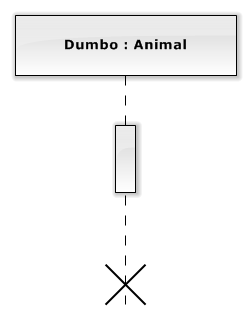
\includegraphics[width=0.3\textwidth]{img/aktivacios_eletvonal.png}
						\caption{Aktivációs életvonal}
					\end{figure}
				\item[Üzenet] \hfill \\
					Az üzenet az objektumok közötti információátadás formája. Az üzenet küldésének az a célja, hogy az objektum működésbe hozza a másik objektumot. Az üzenet azok között az objektumok között jöhet létre, amelyek az objektumdiagramban kapcsolatban állnak. Az üzenetnek van azonosítója (neve, szövege), lehet paramétere, sorszáma.
					
			\end{description}
		\subsection{Együttműködési diagram}
			Az együttműködési diagram azt hivatott bemutatni, hogy miként működnek együtt az osztályok objektumai, milyen üzenetek cseréje révén valósul meg ez az együttműködés.
			(Csak azok az objektumok relevánsak, amelyek osztályait az osztálydiagramban asszociációs kapcsolat köt össze. A diagram mutatja ezt az összekapcsolást és az ehhez tartozó
			üzenetváltásokat, ezért az együttműködési diagram az objektumdiagram bizonyos értelemben vett kiterjesztésének tekinthető.)
			
			Az üzenet küldését egy nyíl mutatja, amely az asszociáció mellett kap helyet és a címzett irányába mutat. Az üzenet azonosítója a nyíl mentén helyezkedik el. Az üzenetnek lehet argumentuma és eredménye. Ezeket egy kis körből induló nyíl mellett helyezzük el, ahol a nyíl az információ áramlásának irányát mutatja.
			
			
		\subsection{Tevékenységdiagram}
			A tevékenységdiagram (aktivációs diagram) a probléma megoldásának lépéseit szemlélteti, a párhuzamosan zajló vezérlési folyamatokkal együtt.
			
			Ha egy tevékenységet
			egy másik tevékenység követ közvetlenül, akkor a két tevékenységet
			nyíllal kötjük össze. Ha adatot (objektumot) ad át egy tevékenység
			egy másik tevékenységnek, akkor a küldő tevékenységből szaggatott
			nyíl vezet az objektumot reprezentáló téglalaphoz, és a téglalaptól
			szaggatott nyíl mutat a fogadó tevékenységre. A téglalapban szögletes
			zárójelek között megadhatjuk az objektum állapotát, státuszát is.
			\begin{figure}[H]
				\centering
				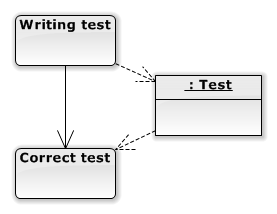
\includegraphics[width=0.3\textwidth]{img/tevekenyseg.png}
				\caption{Objektum átadás}
			\end{figure}
			
			Lehetőség van arra, hogy bizonyos feltételek teljesülése esetén eltérő
			tevékenységeket hajtsunk végre, illetve tevékenységek végrehajtását
			feltételekhez kössük. Ekkor egy rombuszt kell elhelyeznünk a diagramban,
			amelyből kivezető nyilakra írjuk a feltételeket.
			
			\begin{figure}[H]
				\centering
				\includegraphics[width=0.4\textwidth]{img/tevekenyseg2.png}
				\caption{Feltétel ábrázolása}
			\end{figure}
	\section{Használati esetek diagramja}
		A használati esetek diagramja a felhasználók szempontjából kívánja
		szemléltetni azt, hogy a rendszer miként működik, függetlenül attól,
		hogy a szolgáltatásait hogyan valósítja meg.
		
		\noindent
		A diagram részei:
		\begin{itemize}
			\item használati esetek
			\item felhasználók
			\item felhasználási relációk
		\end{itemize}
		
		A használati esetek a rendszer funkcióinak összefoglalásai, szolgáltatási
		egységek. Ez az egység az akcióknak egy olyan sorozata, amelyekkel
		a rendszer a felhasználók egy csoportjával működik együtt.
		
		A használati esetet egy ovális alakzattal jelöljük. A használati eseteket téglalapba foglaljuk, ez jelzi a rendszer határait.
		
		A felhasználók az adott rendszeren kívüli egységek, más programrendszerek,
		alrendszerek, osztályok, illetve személyek lehetnek. Ezek
		aktor szerepet töltenek be. A diagramon egy pálcikaember figurával jelöljük.
		
		A felhasználási relációk kapcsolják össze a használati eseteket a
		felhasználókkal. A relációk egymással is kapcsolatban állhatnak, amit
		a diagramban fel lehet tüntetni. A lehetséges relációk a következők:
		\begin{itemize}
			\item asszociáció \\
				Egy felhasználó és egy használati eset közötti kapcsolatot jelez. (Egyszerű vonal)
			\item általánosítás \\
				Az egyik használati eset a másik általánosabb formája. (Egyszerű vonal, végén fehér háromszöggel)
			\item kiterjesztés \\
				Az egyik használati eset a másikat terjeszti ki. Ennek
				során viselkedéseket illeszt be megadott beszúrási pontoknál. (Szaggatott nyíl $\ll$extend$\gg$ felirattal)
			\item tartalmazás \\
				Az egyik használati eset tartalmazza a másik viselkedését  (Szaggatott nyíl $\ll$include$\gg$ felirattal)
		\end{itemize}
		
		\begin{figure}[H]
			\centering
			\includegraphics[width=0.7\textwidth]{img/hasznalatieset.png}
			\caption{Használati esetek diagramja}
		\end{figure}
\end{document}